\section{Nuclear medicine imaging}
While the previous imaging modalities mostly focused on obtaining static images
of the patient, nuclear medicine imaging concentrates on so-called functional
imaging: visualizing some kind of process (e.g. drug metabolism) in the human
body. CT or MRI scanners also have this capability by exploiting certain side
effects of their underlying phenomena, but the Signal to Noise Ratio (SNR) is
always significantly lower.

Diagnostic nuclear medicine imaging works by tracking radioactive isotopes
(tracers)) as they move through the body. In the early days hospitals needed
their own cyclotron to produce these tracers, which significantly slowed
adoption. Nowadays various companies deliver the needed tracers daily to
hospitals around the world \cite{petreview}. Other variants of nuclear medicine
are used in the oncology departments to fight cancer, but we will not go deeper
into that.

Two main scanner types fall under nuclear medicine imaging: Positron Emission
Tomography (PET) and Single Photon Emission Computer Tomography (SPECT). The
exact difference will be explained later on in the technical background section.
\autoref{fig:petscanner} shows an example of a PET scanner.

\begin{figure}[ht]
\begin{center}
  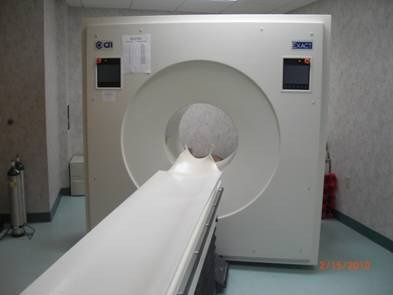
\includegraphics[width=\linewidth]{img/petscanner.jpg}
  \caption{A PET scanner made by Siemens. The opening is completely surrounded
  by detectors, so there are no moving parts inside.}
  \label{fig:petscanner}
\end{center}
\end{figure}

\subsection{History}
The history of nuclear medicine begins with the work of German physicist Hans
Geiger, a student of Ernest Rutherford, and his 1908 invention: the Geiger
counter. This device can detect ionizing radiation by exploiting the fact that
these rays can make an inert gas (e.g. Argon) conduct electricity. Using
this rudimentary device, researchers could form a rough picture of the radioactive
activity in a patient's body \cite{specthistory, geigercountertube}.

A significant breakthrough came with the invention of the Anger camera (or
gamma camera) in 1957 by Hal Anger, an American engineer and physicist. This
camera was able to detect incoming radiation from a whole organ at once,
improving the spatial resolution dramatically. The technique he used was based
on scintillator crystals \cite{anger}.

From there, several researchers such as Crandall, Cassen, Kuhl and Edwards built
upon the work to create true scanner systems throughout the late 1960's and
early 1970's. The first systems were SPECT scanners to make images in just one
plane, and later on CT-like scanners that could calculate cross sections were
invented.

Research concerning PET scanners was performed at about the same time
as SPECT scanners. Scientists soon realised their advantage, but adoption took
much longer in comparison \cite{petreview}. G. Brownell and his group were the
first to build a working dual planar PET scanner \cite{brownell}.

\subsection{Technical background}
Before we explain how PET and SPECT scanners work, we will quickly refresh some
important radioactive decay modes.

The first is positron emission, also called $\beta^+$ decay. Positrons (e$^+$)
are the anti-particles of electrons (e$^-$). During this decay, a proton (p$^+$)
inside an atom is essentially transformed into a neutron (n) and a positron.

\begin{equation}
	p^+ \rightarrow n + e^+
\end{equation}

\begin{equation}
	{}_Z^AX \rightarrow {}_{Z-1}^AY + e^+
\end{equation}

In the next couple of nanoseconds, the positron will fly into a electron and
annihilate. The mass of the two particles is is converted into pure energy in
the form of two photons ($\gamma$). Each photon carries 511 keV of energy and
they fly away in opposite directions.

This physical phenomenon forms the basis of Positron Emission Tomography (PET).
A typical element used during such studies is $^{18}$F, which has a half-life of
about 110 minutes. It yields stable $^{18}$O \cite{suetens}. The fact that two
photons are emitted is very convenient. If both happen to be detected, we
immediately know their projection line. (Remember that in CT scanners the
projection line is known a priori and is fixed between source and detector.)

The opposite operation is also possible: $\beta^-$ decay by electron emission.
Here, a neutron is converted into a proton and an electron.

\begin{equation}
	n \rightarrow p^+ + e^-
\end{equation}

\begin{equation}
	{}_Z^AX \rightarrow {}_{Z+1}^AY + e^-
\end{equation}

In certain cases, the resulting Y atom is in a metastable state ($^{Am}$Y).
This means the atom will later decay further into a more stable nuclear
configuration, releasing one or more photons in the process. This is much more
interesting diagnostic-wise, because unlike electrons, photons don't damage the
tissue they pass through during emission. A common metastable element
used is $^{99m}$Tc, generated after decay of $^{99}$Mo and with further decaying
into $^{99}$Tc (half-life of six hours) by decaying a single photon of 140 keV.

%electron capture

$\beta^-$ decay is mainly used in SPECT scanners. Because only one photon is
emitted, we cannot immediately tell where it came from when it is detected. To
solve this, a mechanical collimator - a thick lead plate with holes in it - is
used to absorb all photons that do not approximately fly perpendicular to it.
Knowing this, we can estimate the projection line of the photons we managed to
detect after they passed through the plate. Sadly, this technique forces us to
make a trade-off between spatial resolution (using smaller holes) and
sensitivity (letting more photons through using bigger holes). This is a serious
disadvantage compared to PET, in turn making SPECT less future-proof.

Note that these photons form electromagnetic waves, and their frequencies are
equal to or higher than those of the X-rays in earlier sections. This means that
they obey the same physical laws, and thus they also attenuate when passing
through tissue. However, in this context we refer to the radiation as
$\gamma$-rays instead.

When the photons are detected and the projection lines are calculated, we have
two options. Either we are satisfied with planar imaging to get a result similar
to basic radiography. In this case all depth information is lost, and the pixels
simply give information about the photon emission activity on their entire
projection line, combined with the attenuation properties of tissue on that
line. Sometimes a SPECT scanner is simply called a gamma camera in this
configuration, although the distinction is mostly theoretical. The other option
is to use a slightly adapted filtered back projection algorithm to compute
CT-like slices. Obviously this requires the detectors to rotate about the
patient just like in a CT scanner.

The detectors used here differ significantly from those used with X-rays. Not
only are there far fewer photons to be detected in the first place, but the
acquisition time is also much longer. Photomultiplier Tubes (PMT) combined with
NaI(Tl) scintillator crystals and, more recently, photo diodes are
popular detectors in use today.

\subsection{Recent advancements}
Due to the strong attenuation of the photons, filtered back projection produces
significant artifacts in the final image. The images are still diagnostically
relevant, but better methods are available. Iterative reconstruction based on
Bayesian statistics or maximum likelihood calculations are becoming more
popular.

Another advancement, the Time-of-Flight (TOF) PET scanner estimates the
source location of the photon along the projection line by measuring the
difference in arrival time of the two photons. This only works reliably if the
difference is smaller than 1ns, which in turn requires very advanced measuring
equipment.

While most researchers focus on nuclear medicine alone, others seek their
fortune in hybrid scanners. For example, combining CT or MRI with PET or SPECT
scanners significantly improves the specificity compared to their stand-alone
versions. Especially the PET/CT combination is popular in clinical environments.
In this case, the CT scanner can provide the attenuation correction needed for
the PET scanner. One problem that has to be overcome is the long acquisition
time needed for PET, and the mismatch it causes with CT scans due to patient
movement. Image registration techniques can be helpful here, but are not
straightforward.
\ldots

\subsection{Future expectations}
As with all types of scanners, we expect steady technological advancements in
the years and decades to come. However, in the case of nuclear medicine, experts
expect most progress to be made on the tracer front. This will enable researcher
to not only visualize biological processes on a macro level, but move to the
molecular level. This way, advanced studies on gene regulation, radio
immunotherapy etc. will become possible.